\section{Motivation and Characterization}
\label{sec:motivation}

% % We study LLM serving on a heterogeneous GPU platform where prefill and decode can be executed on different pools. 
% This section studies LLM serving on a two-pool heterogeneous deployment where prefill and decode can be assigned to different GPU types.
% The goal is to identify the system properties that make energy-efficient scheduling nontrivial in this setting. 
% % It identifies the system properties that make energy-efficient scheduling nontrivial in this setting.
% We first show that hardware heterogeneity makes the most energy-efficient placement phase-dependent: prefill and decode favor different GPU types under different latency budgets.
% We then show that routing, DVFS, tensor parallelism, and active capacity interact in a non-separable manner, so the best setting for one control knob depends on the others. 
% % Together, these observations motivate SWEEP-LLM as a state-aware scheduler that jointly controls routing, parallelism, frequency, and capacity across heterogeneous GPU pools.
% These properties rule out simple static or decomposed strategies, and motivate SWEEP-LLM as a state-aware scheduler that jointly optimizes routing, parallelism, frequency, and capacity across heterogeneous GPU pools.

This section characterizes why energy-efficient LLM serving is difficult on a two-pool heterogeneous deployment where prefill and decode may run on different GPU types. 
We make two observations. 
First, even when prefill and decode are isolated, the energy-minimizing feasible GPU--frequency choice depends on the phase, workload, and latency budget. 
Second, once routing is allowed, it interacts with tensor parallelism, GPU frequency, and active capacity, so the four controls cannot be optimized independently. 
Together, these observations motivate SWEEP-LLM as a state-aware scheduler that jointly optimizes routing, parallelism, frequency, and capacity across heterogeneous GPU pools.

% Three observations, each motivating a specific SWEEP-LLM design element that goes beyond DynamoLLM:
% Obs 1: Heterogeneous hardware creates phase-specific efficiency regions (Exp C + D + B_shared)

% L40S prefill TTFT is 33× faster than L4 for il=1024 — hardware-forced prefill assignment
% L4 decode hits a sharp frequency plateau at 1410 MHz: TPOT is flat from 1410→2040 MHz, so running at 990 MHz saves up to 57% decode energy with zero latency penalty
% L4 TP=2 at 990 MHz is 20% more energy-efficient than the best L40S TP=1 for balanced workloads
% Motivates: heterogeneous pool design + phase-aware routing (DynamoLLM can't show this — single GPU type)

% Obs 2: Routing, TP, frequency, and allocation interact across pools (Exp A + C + D)

% Once you route prefill to L40S, the optimal L40S freq depends on prefill load (frequency-sensitive at low load, saturated at high load)
% Once you route decode to L4, the optimal L4 freq is always 990–1200 MHz regardless of load (the plateau)
% Changing routing changes pool loads, which changes the optimal TP and freq per pool
% Motivates: joint optimization rather than DynamoLLM's hierarchical decomposition

% Obs 3: Disaggregation benefit is conditional, not automatic (Exp E + A + B)

% TCP-based KV transfer adds ≥8s TTFT — disaggregation is strictly worse under this infrastructure
% Even with fast transfer, the scheduler must weigh disaggregation gain against coordination overhead per workload
% Motivates: the scheduler must decide when to disaggregate, not always disaggregate
% This structure makes every observation about something DynamoLLM cannot address due to its homogeneous, non-disaggregated setting. No redundancy.


% [OLD Observation 1 — removed: DynamoLLM (HPCA'25) already establishes that
% no single (TP, freq) is universally energy-optimal across workloads on
% homogeneous clusters (their Insight #1, Table I).  Repeating the claim on
% L40S adds little.  The new Obs 1 instead targets what DynamoLLM cannot
% show: heterogeneous hardware with phase-specific efficiency regions.]
%
% \subsection{Observation 1: No Universal Operating Point}
% \label{sec:motivation:no-universal-optimum}
%
% \begin{figure*}[t]
%   \centering
%   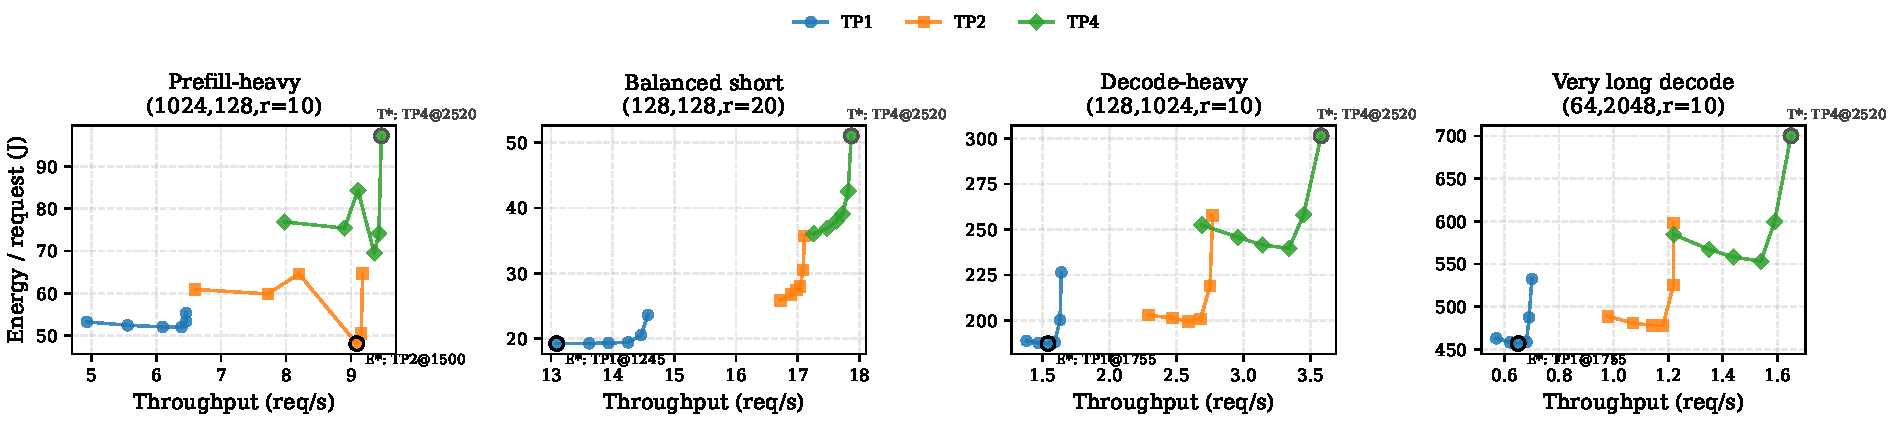
\includegraphics[width=\textwidth]{figures/figA_no_universal_optimum.pdf}
%   \caption{Experiment \texttt{A} on monolithic L40S.
%   Each point is one $(\mathrm{TP}, f)$ configuration.
%   The throughput-optimal point and the energy-optimal point diverge in all four representative workloads.
%   The energy-optimal point also shifts with workload.}
%   \label{fig:a-no-universal-optimum}
% \end{figure*}
%
% Experiment \texttt{A} isolates the simplest version of our scheduling problem by running monolithic vLLM on a single GPU type, the L40S, while sweeping workload, TP degree, and SM frequency.
% Fig.~\ref{fig:a-no-universal-optimum} shows four representative workloads from experiment \texttt{A}: prefill-heavy $(1024,128,r{=}10)$, balanced short $(128,128,r{=}20)$, decode-heavy $(128,1024,r{=}10)$, and very long decode $(64,2048,r{=}10)$.
% In all four cases, the highest-throughput point is TP4 at $2520$\,MHz, but that operating point is not energy-optimal.
% The energy-optimal point is TP2 at $1500$\,MHz for the prefill-heavy workload, TP1 at $1245$\,MHz for the balanced short workload, and TP1 at $1755$\,MHz for both decode-heavy workloads.
% Relative to the energy-optimal point, selecting the throughput-optimal point increases energy per request by $2.02\times$ for $(1024,128,r{=}10)$, $2.66\times$ for $(128,128,r{=}20)$, $1.61\times$ for $(128,1024,r{=}10)$, and $1.53\times$ for $(64,2048,r{=}10)$.
% Therefore, even before introducing heterogeneity or disaggregation, a fixed monolithic configuration is insufficient to optimize both throughput and energy across workloads.
% This observation motivates workload-aware control in SWEEP-LLM rather than a single static operating point.

% \subsection{Observation 1: Heterogeneous Hardware Creates Phase-Specific Efficiency Regions}
% \label{sec:motivation:heterogeneity}

% \begin{figure*}[t]
%   \centering
%   \begin{minipage}[t]{0.49\textwidth}
%     \centering
%     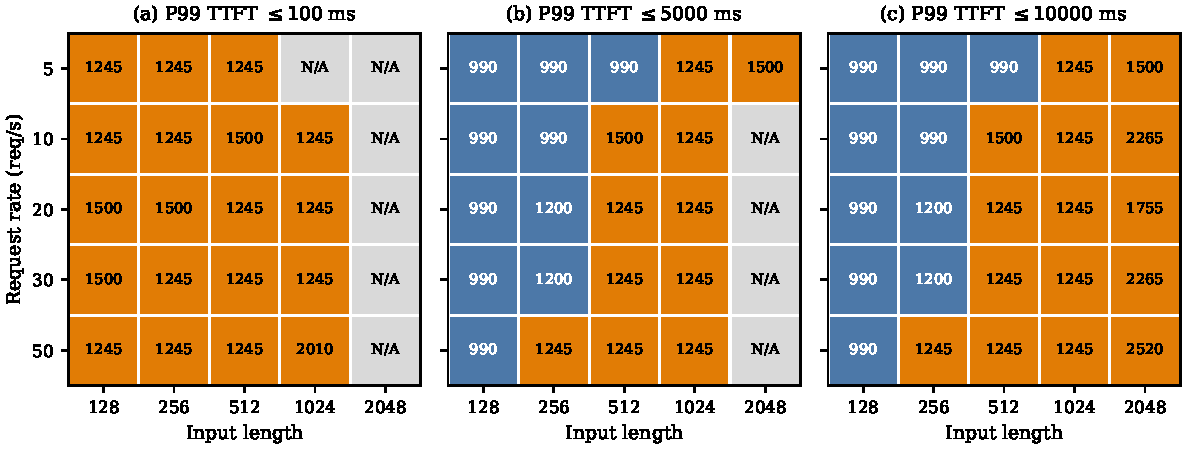
\includegraphics[width=\linewidth]{figures/fig_obs1_prefill_slo_regions_info_to_end_p99.pdf}
%   \end{minipage}\hfill
%   \begin{minipage}[t]{0.49\textwidth}
%     \centering
%     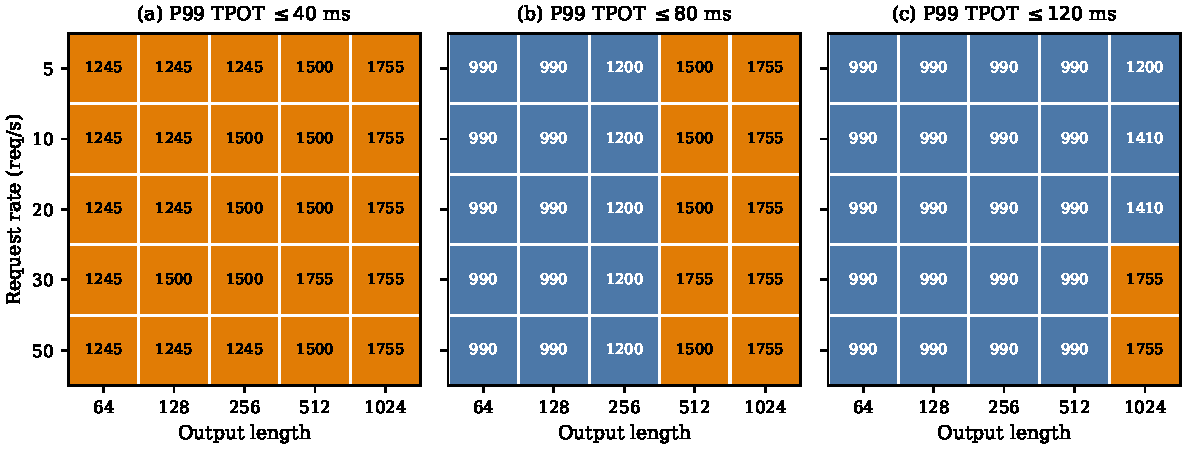
\includegraphics[width=\linewidth]{figures/fig_obs1_decode_slo_regions_info_to_end_p99.pdf}
%   \end{minipage}
%   \vspace{0.2em}

%   {\footnotesize
%   \textcolor[rgb]{0.298,0.471,0.659}{\rule{1.2em}{1.2ex}}\ L4 wins\quad
%   \textcolor[rgb]{0.882,0.486,0.020}{\rule{1.2em}{1.2ex}}\ L40S wins\quad
%   \textcolor[rgb]{0.851,0.851,0.851}{\rule{1.2em}{1.2ex}}\ No feasible config\par}
%   \caption{Observation 1 from experiments \texttt{C}/\texttt{C$'$} and \texttt{D}/\texttt{D$'$}.
%   Tensor parallelism is fixed at $\mathrm{TP}{=}1$ in these phase-only experiments.
%   Each cell shows the hardware-frequency pair that minimizes energy per request subject to the indicated \emph{P99} latency bound.
%   Energy is computed from the first benchmark-log \texttt{INFO} timestamp to the end of the monitor trace.
%   Infeasible cells marked \texttt{N/A} mean that no measured configuration in the corresponding $\mathrm{TP}{=}1$ sweep satisfies that SLO.
%   Tight TTFT bounds push prefill toward the L40S, whereas relaxed TPOT bounds make decode increasingly favor the L4.}
%   \label{fig:obs1-phase-regions}
% \end{figure*}

% Prior work has already shown that heterogeneous request mixes break any single energy-optimal operating point on a homogeneous cluster~\cite{stojkovic2024dynamollm}.
% Our setting adds a different question: whether phase placement itself changes the energy-optimal hardware once \emph{tail-latency} constraints are enforced.
% Experiments \texttt{C}/\texttt{C$'$} and \texttt{D}/\texttt{D$'$} isolate prefill and decode on both GPU types, and Fig.~\ref{fig:obs1-phase-regions} summarizes the resulting winner regions using P99 TTFT/TPOT and INFO-to-end energy accounting.

% The decode pattern is the clearest.
% Under a strict P99 TPOT budget of $40$\,ms, all 25 workloads select the L40S.
% At $80$\,ms, the winner map splits, with 15 workloads moving to the L4 and 10 remaining on the L40S.
% At $120$\,ms, 23 workloads select the L4 and only 2 remain on the L40S.
% For example, at $(\mathrm{ol}{=}1024,r{=}10)$, the best feasible point shifts from L40S at $1755$\,MHz under $\mathrm{TPOT}\leq 40$\,ms to L4 at $1410$\,MHz under $\mathrm{TPOT}\leq 120$\,ms.
% Thus decode exhibits a clean latency-energy tradeoff: L40S is required when TPOT is tight, but L4 is preferred once the latency budget relaxes.

% Prefill is more regime-dependent.
% Under P99 $\mathrm{TTFT}\leq 100$\,ms, 19 workloads select the L40S and 6 are infeasible in the measured $\mathrm{TP}{=}1$ sweep.
% At $\mathrm{TTFT}\leq 5000$\,ms, the map becomes mixed, with 10 L4 winners, 11 L40S winners, and 4 infeasible workloads.
% At $\mathrm{TTFT}\leq 10000$\,ms, all 25 workloads become feasible, but the L40S still leads 15 to 10.
% The boundary remains sharp even at fixed prompt length: for $(\mathrm{il}{=}128,r{=}10)$ the winner stays on L40S at $1245$\,MHz under $\mathrm{TTFT}\leq 100$\,ms, while for the same prompt length under $\mathrm{TTFT}\leq 5000$\,ms the winner moves to L4 at $990$\,MHz.

% These results establish phase-specific energy-latency regions rather than a simple hardware ranking.
% Decode moves decisively from L40S to L4 as the TPOT budget relaxes, whereas prefill shifts more gradually and remains sensitive to both prompt length and offered load.
% This asymmetry is the reason SWEEP-LLM separates the pools and makes routing phase-aware instead of treating the two GPU types as interchangeable.
% For these SLO-constrained phase-only views, tensor parallelism remains fixed at $\mathrm{TP}{=}1$, and an \texttt{N/A} cell means that no measured configuration in that $\mathrm{TP}{=}1$ sweep satisfies the corresponding latency bound.


% \subsection{Observation 1: Heterogeneity makes the energy-optimal placement phase-dependent}
\subsection{Phase-dependent Optimal Placement}
\label{sec:motivation:heterogeneity}

Prior work has shown that no single operating point minimizes energy across all request mixes on a homogeneous cluster~\cite{stojkovic2024dynamollm}. 
Heterogeneous, phase-disaggregated serving adds a more basic placement question: once prefill and decode may run on different GPU types, does the energy-minimizing feasible device depend on the phase, workload, and latency budget?
To isolate hardware and frequency effects, we run prefill-only and decode-only serving on a single NVIDIA L40S and a single NVIDIA L4 with $\mathrm{TP}{=}1$, sweeping GPU frequency. 
For each workload--SLO pair, we select the lowest-energy configuration on each GPU that satisfies the corresponding tail-latency bound, then compare the two winners. 
Figure~\ref{fig:obs1-phase-regions} reports the resulting hardware--frequency winner maps for isolated prefill and decode.

The winner regions change substantially with both phase and latency budget. 
Decode shows the clear transition: under a tight $\mathrm{TPOT}\leq 40$\,ms bound, all 25 measured workloads select the L40S; when the bound is relaxed to $80$\,ms, 15 workloads shift to the L4 and 10 remain on the L40S; at $120$\,ms, 23 of 25 workloads select the L4. 
Prefill transitions more gradually. 
Under $\mathrm{TTFT}\leq 100$\,ms, 19 workloads select the L40S and 6 are infeasible in the measured $\mathrm{TP}{=}1$ space. 
At $\mathrm{TTFT}\leq 5000$\,ms, the map becomes mixed (10 L4 winners, 11 L40S winners, and 4 infeasible workloads), and at $\mathrm{TTFT}\leq 10000$\,ms all workloads become feasible, though the compute-oriented L40S still wins 15 of 25 cases.

These measurements show that heterogeneity does not induce a fixed global GPU ranking. 
Decode can move from L40S to L4 as the TPOT budget relaxes, whereas larger prefills often remain better matched to the L40S even under looser TTFT bounds. 
Thus an energy-efficient scheduler must treat phase placement as a runtime decision, not a static assignment. 
This motivates SWEEP-LLM's explicit routing control, and the next subsection shows that routing must then be coordinated with TP, frequency, and active capacity rather than optimized independently.


% Prior work on homogeneous clusters has shown that no single operating point minimizes energy across all request mixes~\cite{stojkovic2024dynamollm}.
% % Our setting extends this observation to heterogeneous platforms: once prefill and decode can be placed on different GPU types, the energy-optimal placement itself becomes phase-dependent under latency constraints.
% In a heterogeneous deployment, a further question arises: once prefill and decode can be assigned to different GPU types, does the most energy-efficient hardware choice itself become phase- and SLO-dependent?
% % this observation extends to phase placement itself: once prefill and decode can be assigned to different GPU types, the energy-optimal placement becomes phase-dependent under latency constraints.
% % To isolate this effect, we run prefill-only and decode-only serving separately on a single L40S and a single L4, fix $\mathrm{TP}{=}1$, sweep GPU frequency, and, for each workload--SLO pair, compare the minimum-energy feasible operating point on the two GPUs. 
% To isolate this effect, we run prefill-only and decode-only serving on a single NVIDIA L40S GPU and a single NVIDIA L4 GPU at $\mathrm{TP}{=}1$, sweeping GPU frequency. 
% For each workload--SLO pair, we then compare the minimum-energy feasible operating point on the two GPUs.
% Figure~\ref{fig:obs1-phase-regions} summarizes the winning hardware--frequency choice for isolated prefill and decode across the measured workloads and SLOs.

% Both prefill and decode exhibit a pronounced hardware transition as the SLO budget relaxes.
% For decode under a strict $\mathrm{TPOT}\leq 40$\,ms bound, all 25 measured workloads select the L40S.
% When the bound is relaxed to $80$\,ms, 15 workloads shift to the L4 and 10 remain on the L40S.
% At $120$\,ms, 23 of the 25 workloads select the L4.
% For prefill under a tight $\mathrm{TTFT}\leq 100$\,ms bound, 19 workloads select the L40S and the remaining 6 are infeasible in the measured $\mathrm{TP}{=}1$ space.
% At $\mathrm{TTFT}\leq 5000$\,ms, the winner map becomes mixed, with 10 L4 winners, 11 L40S winners, and 4 infeasible workloads.
% At $\mathrm{TTFT}\leq 10000$\,ms, all 25 workloads become feasible, yet the L40S still leads by 15 workloads to 10.
% Compared with decode, the prefill boundary is less uniform and larger prefills remain better matched to the compute-oriented L40S.
% These results establish that heterogeneity creates phase-specific efficient regions, and the energy-efficient device--frequency pair depends directly on the workload and SLO budget. 


\subsection{Joint Optimization}
\label{sec:motivation_joint}

% Observation~1 established that phase placement is itself workload- and SLO-dependent.
% The follow-up question is whether the remaining control knobs (intra-pool DVFS, TP, and active capacity) can be tuned independently once routing is phase-aware, or whether their optima are coupled and must be chosen together.
To study how routing, DVFS, TP, and active capacity interact, we construct two controlled workload states with the same aggregate arrival rate ($2$ requests/s) and the same latency bounds ($\mathrm{TTFT}\leq 500$ ms, $\mathrm{TPOT}\leq 200$ ms), but opposite phase balance. 
Each state mixes request classes of differing length, labelled by (input, output) with S/M/L denoting $128/1024/2048$ input and $128/512/1024$ output tokens. 
% These three levels are chosen to span a realistic prompt-length range and are independent of the coarser request taxonomy used by the runtime scheduler (\S\ref{sec:request_classes}). 
The prefill-heavy state combines short, moderate, and long prompts with short generations ($30\%$ SS, $40\%$ MS, $30\%$ LS), whereas the decode-heavy state comprises $30\%$ SL, $25\%$ MM, $25\%$ LS, $20\%$ SS.
% This length spread mirrors the production traces used in \S\ref{sec:eval}, whose prompts range from a hundred to several thousand tokens.
For each state, we compare six policies in an increasingly rich control space. 
\textsc{Static-disagg} fixes prefill on L40S, decode on L4, maximum frequency, $\mathrm{TP}{=}1$, and all GPUs active. \textsc{Route-only}, \textsc{Route+DVFS}, and \textsc{Route+DVFS+TP} progressively add one control dimension while keeping the remaining dimensions fixed. 
Finally, we compare two controllers with the same four-knob space: a hierarchical \textsc{Sequential} policy that commits the knobs one stage at a time, and \textsc{Full joint} optimization. 
To avoid penalizing \textsc{Sequential} for an arbitrary knob order, we report its best result over all $24$ possible stage orderings. 
Figure~\ref{fig:motivation_joint} reports the resulting energy comparisons across the six scheduling policies and the configurations selected for the two workload states.


% \begin{table}[!t]
%     \centering
%     \caption{Selected \textsc{Full} joint configurations for the two workload states in Fig.~\ref{fig:motivation_joint}.}
%     \label{tab:obs2-full-joint-configs}
%     \scriptsize
%     \setlength{\tabcolsep}{6.3pt}
%     \renewcommand{\arraystretch}{1}
%     \begin{tabular}{@{}lccccccc@{}}
%         \toprule
%         State & Route & $f_{\mathrm{L40S}}$ & $f_{\mathrm{L4}}$ & $TP_{\mathrm{L40S}}$ & $TP_{\mathrm{L4}}$ & $Act_{\mathrm{L40S}}$ & $Act_{\mathrm{L4}}$ \\
%         \midrule
%         Prefill-heavy & \textbf{A$\rightarrow$A} & \textbf{1500} & \textbf{780} & 1 & \textbf{1} & \textbf{2} & \textbf{0} \\
%         Decode-heavy  & \textbf{A$\rightarrow$B} & \textbf{2010} & \textbf{1200} & 1 & \textbf{4} & \textbf{1} & \textbf{4} \\
%         \bottomrule
%     \end{tabular}
% \end{table}

\begin{figure*}[!t]
    \vspace{-0.5cm}
    \centering
    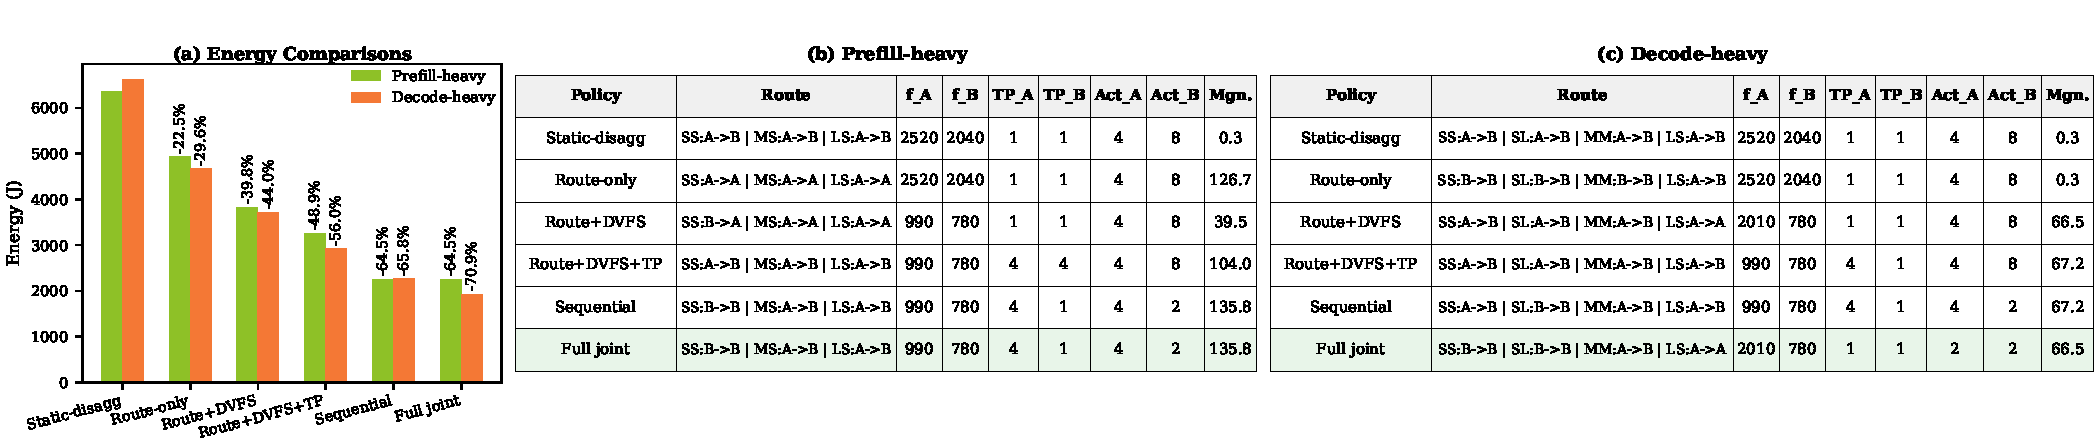
\includegraphics[width=\textwidth]{figures/obs2_regime_search_primary/r2_ttft500_tpot200_mixedlen_obs2_main.pdf}
    \vspace{-0.8cm}
    \caption{
      % Prefill-heavy and decode-heavy states at $2$\,requests/s under $\mathrm{TTFT}\leq 500$\,ms and $\mathrm{TPOT}\leq 200$\,ms.
      (a) Energy comparisons across progressively larger control spaces, with labels giving the reduction relative to the \textsc{Static-disagg} baseline.
      (b--c) The selected configurations for the two states. 
      % Request classes are labelled by (input, output) length, with S/M/L ${=}\,128/1024/2048$ input and $128/512/1024$ output tokens (e.g., LS is a $2048$-token prompt with a $128$-token output). 
      Mgn.\ is the smallest margin to the TTFT or TPOT bound across all classes (ms); A and B denote the L40S and L4 pools.
      This is a model-predicted controlled study built from hardware-calibrated per-configuration models; it illustrates knob coupling rather than validating end-to-end deployment performance.
      % Table~\ref{tab:obs2_hw_validation} spot-checks the underlying per-configuration mechanisms on the real L40S/L4 testbed.
      % The selected route, frequency, tensor parallelism, and active capacity all vary across policies, and the full-joint optimum differs substantially across the two workload states.
      }
    \label{fig:motivation_joint}
\end{figure*}


Figure~\ref{fig:motivation_joint}(a) first shows that expanding the control space exposes large energy savings over the fixed deployment. 
In the prefill-heavy state, the ordered additions of per-class routing, DVFS, TP, and active-capacity control reduce energy by $22.5\%$, a further $22.4\%$, another $15.0\%$, and a final $30.7\%$, for a cumulative $64.5\%$ reduction over \textsc{Static-disagg}. 
The decode-heavy state follows the same pattern ($29.6\%$, $20.5\%$, $21.4\%$, and $33.9\%$; $70.9\%$ cumulative). 
These numbers represent an ordered control-space expansion, not independent marginal contributions: the value of each knob depends on which other knobs are already available. 
The experiment shows that restricting the scheduler to any single control dimension leaves substantial energy on the table.

Next, we compare \textsc{Sequential} and \textsc{Full joint}, which have access to the same four controls. 
In the prefill-heavy state, the best sequential ordering happens to match the joint solution. 
In the decode-heavy state, however, \textsc{Sequential} remains $14.8\%$ higher in energy than \textsc{Full joint}. 
The reason is that routing and TP are coupled: the low-energy feasible point requires choosing which classes stay within one pool, which classes cross pools, and how much parallelism each pool uses as one combined decision. 
Once a sequential policy commits an early routing or TP choice, later stages cannot always recover the globally better capacity-frequency trade-off.

Figure~\ref{fig:motivation_joint}(b)--(c) illustrates this coupling. 
In the prefill-heavy state, \textsc{Full joint} sends the moderate and long-prompt classes through the L40S prefill path (MS and LS via A$\rightarrow$B), uses $TP_A{=}4$ at a low L40S frequency ($990$ MHz), and serves the short class together with decode on two L4 GPUs at $TP_B{=}1$ and $780$ MHz. 
In the decode-heavy state, the solution changes on every axis: L40S uses lower TP but a higher frequency ($TP_A{=}1$, $f_A{=}2010$ MHz on two GPUs), long-generation traffic is concentrated on L4, and the light-decode long-prompt class keeps decode on L40S (A$\rightarrow$A) to avoid cross-pool KV transfer. 
% These two feasible low-energy configurations cannot be described by a fixed phase split, a fixed TP choice, or a fixed frequency policy.

% \noindent\textit{Every knob contributes, and joint search strictly dominates hierarchical.}
% Fig.~\ref{fig:motivation_joint}(a) shows that the \textsc{Static-disagg} deployment, although feasible, is far from energy-efficient: it runs both pools at maximum frequency with all GPUs active and only just meets the SLO.
% Enlarging the control space reduces energy monotonically. 
% In the prefill-heavy state, per-class routing saves $22.5\%$, DVFS a further $22.4\%$, tensor parallelism another $15.0\%$, and active-capacity control a final $30.7\%$, a cumulative $64.5\%$ over \textsc{Static-disagg}; the decode-heavy state follows the same pattern ($29.6\%$, $20.5\%$, $21.4\%$, and $33.9\%$; $70.9\%$ cumulative). 
% Every knob contributes, and the single largest step is active capacity, which powers down the GPUs the fixed-capacity policies are forced to leave idle (e.g., Route+DVFS+TP keeps all eight L4 GPUs powered, four of them idle).
% Next, we compare the \textsc{Full Joint} with the decomposed \textsc{Sequential} policy. 
% In the prefill-heavy state, the best of all $24$ stage orderings happens to match the joint solution, but in the decode-heavy state the \textsc{Sequential} policy falls short by $14.8\%$, because here routing and tensor parallelism must be chosen together.
% Since a controller cannot know in advance which state permits decomposition, only joint search is reliably optimal.

% Fig.~\ref{fig:motivation_joint}(b)--(c) shows that the two selected configurations place work very differently across the heterogeneous pools.
% % , yet both rely on the L40S for long-prompt prefill (no all-L4 configuration is feasible for these prompts). 
% In the prefill-heavy state, \textsc{Full joint} consolidates the long and moderate prefill (LS and MS, via A$\rightarrow$B) onto four L40S GPUs at $TP_A{=}4$, $f_A{=}990$\,MHz, and serves the short class together with all decode on just two L4 GPUs ($TP_B{=}1$, $f_B{=}780$\,MHz). 
% In the decode-heavy state the allocation differs on every axis: the L40S carries less prefill, so it trades parallelism for clock speed ($TP_A{=}1$, $f_A{=}2010$\,MHz on two GPUs) to meet the long-prompt TTFT; the long-generation class (SL) is served entirely on the L4; and the light-decode long-prompt class (LS) keeps its decode on the L40S (A$\rightarrow$A) to avoid a cross-pool KV transfer. 
% In both states the L4 runs at a lower frequency ($f_B{=}780$\,MHz): the prefill routed to it comes from short prompts, whose TTFT is easily met even at low frequency, while its decode is memory-bound and does not benefit from a higher clock, so a reduced frequency minimizes the pool's energy while still meeting both bounds.

Together, these results show why the scheduling problem is non-separable. 
% Together, these results demonstrate that the four knobs are coupled and rule out any fixed configuration and decomposed per-knob tuning.
Routing determines which pool sees prefill and decode load; TP determines the per-instance capacity and how many instances fit; frequency changes both latency and power; and active-capacity control determines how much idle power can be eliminated.
Since the best setting of one knob depends on the others and changes with workload state, SWEEP-LLM uses state-aware joint search rather than decomposed per-knob tuning.
% show that decomposed per-knob tuning cannot be relied upon: it matches the joint solution in some states but not in others, and a controller cannot tell in advance which case it faces.
% We show that the four knobs are coupled: routing dictates the feasible tensor parallelism, which in turn sets the most energy-efficient frequency and the number of pools worth powering. 
% The joint solution, including which pools are active at all, shifts with the workload state.
% This motivates SWEEP-LLM's state-aware joint search, which reconsiders routing, DVFS, tensor parallelism, and active capacity together whenever the workload state transitions.



% \paragraph{Grounding the model-predicted study.}
% Fig.~\ref{fig:motivation_joint} is a model-predicted controlled study, not a direct end-to-end hardware replay. To avoid using the model as an ungrounded motivation, the predictive models are fitted and grouped-cross-validated on real L40S/L4 measurements (\S\ref{sec:phase_a_models}), and we additionally spot-check the key per-configuration mechanisms on the testbed (Table~\ref{tab:obs2_hw_validation}). The most counter-intuitive primitive, that L4 decode at a low clock ($1200$\,MHz) is feasible and low-power (measured TPOT $\approx 24$\,ms at $\approx 279$\,W), holds on real hardware, and the model is conservative there. These spot checks validate the hardware primitives the model composes; the joint-versus-sequential comparison itself is a composition of calibrated per-configuration models rather than a direct hardware replay.

% \begin{table}[t]
% \centering
% \small
% \caption{Hardware spot-validation of the per-configuration mechanisms behind Fig.~\ref{fig:motivation_joint}, measured on the L4 testbed (median of three runs) against the model used to generate the figure. The model is conservative on these cells (it does not under-predict latency). These checks validate per-configuration primitives, not the end-to-end joint-versus-sequential comparison. Generated by \texttt{compare\_obs2\_validation.py}.}
% \label{tab:obs2_hw_validation}
% \begin{tabular}{llrrr}
% \toprule
% Mechanism & Config (L4) & Measured & Model & Power \\
% \midrule
% Low-freq decode & TP4, il32/ol1024, $1200$\,MHz & TPOT $24.2$\,ms & $28.2$\,ms & $279$\,W \\
% feasible \& cheap & TP4, il32/ol1024, $1410$\,MHz & TPOT $24.2$\,ms & $27.9$\,ms & $278$\,W \\
% \midrule
% Prefill freq-flat & TP1, il128/ol32, $1410$\,MHz & TTFT $192$\,ms & $219$\,ms & $62$\,W \\
%  & TP1, il128/ol32, $1755$\,MHz & TTFT $192$\,ms & $219$\,ms & $63$\,W \\
% \bottomrule
% \end{tabular}
% \end{table}


% Prior work has shown that no single GPU configuration is energy-optimal across all LLM workloads on a homogeneous cluster~\cite{dynamollm}.
% SWEEP-LLM targets a heterogeneous setting where two structurally different GPU types are available.
% The key additional question is whether different inference phases map to different hardware, and if so, whether the energy-efficient operating region differs across phases.
% Experiments \texttt{C}/\texttt{C$'$} (prefill-only on L40S/L4) and \texttt{D}/\texttt{D$'$} (decode-only on L4/L40S) isolate each phase on each GPU type, forming a complete $2\times 2$ matrix that reveals three complementary effects.
%
% \paragraph{Prefill is compute-sensitive on L40S at low load but saturates at high load.}
% Experiment~\texttt{C} runs prefill-only serving on the L40S across six frequencies.
% For large prompts ($\mathrm{il}{=}1024$) at low arrival rate ($r{=}5$), increasing frequency from 1245 to 2520\,MHz reduces P99~TTFT by 37\% (from \placeholder{197.6} to \placeholder{123.2}\,ms), confirming that single-request prefill is compute-bound.
% At high load ($r{=}50$), the same frequency sweep reduces TTFT by less than \placeholder{5}\%, because the system is memory-bandwidth-limited once multiple prefills are batched.
% This load-dependent crossover means that a fixed prefill frequency is either wasteful at low load or too slow at high load
% (Fig.~\ref{fig:obs1-phase-efficiency}a).
%
% \paragraph{Decode hits a sharp frequency plateau on L4; L40S decode is faster but costlier.}
% Experiment~\texttt{D} runs decode-only serving on the L4.
% Across all tested output lengths ($\mathrm{ol}\in\{128,256,512,1024\}$) and rates, P99~TPOT is effectively flat above 1410\,MHz: the variation from 1410 to 2040\,MHz is less than 0.3\,ms.
% The autoregressive decode step is memory-bandwidth-bound, so additional SM frequency provides no latency benefit.
% Running at 990\,MHz instead of 2040\,MHz saves up to 57\% energy per request for short outputs ($\mathrm{ol}{=}128$) and 48\% for medium outputs ($\mathrm{ol}{=}256$), with no measurable TPOT penalty.
% Experiment~\texttt{D$'$} runs the same decode-only workloads on the L40S.
% The L40S achieves \placeholder{$M$}$\times$ lower TPOT thanks to its higher memory bandwidth, but at \placeholder{$P$}$\times$ higher power draw.
% When the resulting TPOT on L4 already satisfies the SLO, routing decode to L4 at low frequency is strictly more energy-efficient
% (Fig.~\ref{fig:obs1-phase-efficiency}b).
%
% \paragraph{Large-prompt prefill is hardware-bound to the compute-oriented pool.}
% Experiment~\texttt{C$'$} runs the same prefill-only workloads on the L4.
% For $\mathrm{il}{=}1024$ at $r{=}5$, L4 P99~TTFT is \placeholder{$X$}\,ms versus \placeholder{$Y$}\,ms on the L40S---a \placeholder{$N$}$\times$ gap.
% The L40S's higher FP16 throughput (181\,TFLOPS versus 30\,TFLOPS on the L4) makes it the only viable prefill pool for long prompts under tight TTFT SLOs
% (Fig.~\ref{fig:obs1-phase-efficiency}c).
%
% \paragraph{Energy-efficiency depends on workload shape and SLO.}
% Although the L4 is slower, its lower power draw can make it more energy-efficient when the latency budget permits.
% Experiment~\texttt{B\_shared} (monolithic L4~TP2) versus experiment~\texttt{A} (monolithic L40S~TP1) shows this tradeoff concretely.
% For balanced short requests $(\mathrm{il}{=}128,\mathrm{ol}{=}128)$ at $r{=}10$, L4~TP2 at 990\,MHz consumes 17.27\,J/req versus 27.27\,J/req on the L40S at 1245\,MHz---37\% less energy---while P99~TTFT rises from 109 to 157\,ms, which may still satisfy a 200--500\,ms SLO.
% At $r{=}20$, the gap narrows to 17\% (15.91 versus 19.13\,J/req) as the L40S becomes better utilized.
% Conversely, for long-prompt requests $(\mathrm{il}{=}1024,\mathrm{ol}{=}128)$ at $r{=}10$, L4~TP2 saves only 10\% energy but its P99~TTFT explodes to 6852\,ms (versus 740\,ms on L40S), making it infeasible under any practical SLO.
% The energy-optimal hardware assignment therefore depends on both the request's token shape and the prevailing SLO target.
%
% \medskip
% \noindent
% These results establish that prefill and decode occupy fundamentally different efficiency regions in the (frequency, hardware) space.
% The L40S is indispensable for compute-bound prefill; the L4 is preferable for memory-bound decode at low frequency; and the energy-optimal pool assignment is request-dependent.
% This three-way asymmetry motivates SWEEP-LLM's heterogeneous pool design and phase-aware routing, a dimension absent from prior homogeneous-cluster schedulers~\cite{dynamollm}.

% Prior work has already shown that heterogeneous request mixes break any single energy-optimal operating point on a homogeneous cluster~\cite{stojkovic2024dynamollm}.
% Our setting adds a different question: whether the two inference phases themselves prefer different hardware once latency and energy are considered together.
% Experiments \texttt{C}/\texttt{C$'$} and \texttt{D}/\texttt{D$'$} answer this question by isolating prefill and decode on both GPU types.
% Fig.~\ref{fig:obs1-phase-regions} summarizes the resulting winner regions over the measured token-length and load space.
%
% The resulting pattern is asymmetric.
% For decode, the L4 is the energy winner in all 25 measured workloads.
% For example, at $(\mathrm{ol}{=}1024,r{=}10)$, the best L4 point is $147.3$\,J/request at $108.2$\,ms TPOT, whereas the best L40S point is $184.3$\,J/request at $32.2$\,ms TPOT.
% Thus decode on L4 trades latency for a consistent energy advantage, and its efficient operating region remains concentrated at $990$--$1200$\,MHz.
%
% For prefill, the answer depends on prompt length and load.
% At short prompts, the L4 can still be more energy-efficient.
% However, once the prompt becomes long enough or the offered load increases, the L40S becomes both faster and cheaper.
% At $(\mathrm{il}{=}1024,r{=}10)$, the best L40S point achieves $16.1$\,J/request and $52.3$\,ms TTFT, whereas the best L4 point requires $22.2$\,J/request and $8.39$\,s TTFT.
% Across the measured prefill-only workloads, the L40S is the energy winner exactly in the large-prompt, high-load region where TTFT becomes the binding concern.
%
% These results establish phase-specific energy-latency regions rather than a simple hardware ranking.
% Long, compute-intensive prefills naturally belong on the L40S pool, while decode requests are served most efficiently on the L4 pool when their TPOT remains within budget.
% This asymmetry is the reason SWEEP-LLM separates the pools and makes routing phase-aware instead of treating the two GPU types as interchangeable.
% For the SLO-constrained phase-only views, tensor parallelism remains fixed at $\mathrm{TP}{=}1$, and an \texttt{N/A} cell means that no measured configuration in that $\mathrm{TP}{=}1$ sweep satisfies the corresponding latency bound.

% Prior work has already shown that heterogeneous request mixes break any single energy-optimal operating point on a homogeneous cluster~\cite{stojkovic2024dynamollm}.
% Our setting adds a different question: whether phase placement itself changes the energy-optimal hardware once latency constraints are enforced.
% Experiments \texttt{C}/\texttt{C$'$} and \texttt{D}/\texttt{D$'$} isolate prefill and decode on both GPU types, and Fig.~\ref{fig:obs1-phase-regions} summarizes the resulting SLO-constrained winner regions.
%
% The decode pattern is the clearest.
% Under a strict TPOT budget of $40$\,ms, all 25 workloads select the L40S.
% At $80$\,ms, the winner map splits, with 15 workloads moving to the L4 and 10 remaining on the L40S.
% At $120$\,ms, all 25 workloads select the L4.
% For example, at $(\mathrm{ol}{=}1024,r{=}10)$, the best feasible point shifts from L40S at $1755$\,MHz under $\mathrm{TPOT}\leq 40$\,ms to L4 at $990$\,MHz under $\mathrm{TPOT}\leq 120$\,ms.
% Thus decode exhibits a clean latency-energy tradeoff: L40S is required when TPOT is tight, but L4 is preferred once the latency budget relaxes.
%
% Prefill is more regime-dependent.
% Under $\mathrm{TTFT}\leq 100$\,ms, 19 workloads select the L40S, only one selects the L4, and five are infeasible in the measured $\mathrm{TP}{=}1$ sweep.
% At $\mathrm{TTFT}\leq 5000$\,ms, the map becomes mixed, with 12 L4 winners, 10 L40S winners, and 3 infeasible workloads.
% At $\mathrm{TTFT}\leq 10000$\,ms, all 25 workloads become feasible and the winner counts are nearly balanced at 13 for L4 and 12 for L40S.
% The boundary can be sharp even for the same prompt length: for $(\mathrm{il}{=}128,r{=}10)$, L4 at $1620$\,MHz is the cheapest feasible point under $\mathrm{TTFT}\leq 100$\,ms, whereas for $(\mathrm{il}{=}128,r{=}5)$ no L4 point meets that bound and the winner moves to L40S at $1500$\,MHz.
%
% These results establish phase-specific energy-latency regions rather than a simple hardware ranking.
% Decode moves from L40S to L4 as the TPOT budget relaxes, whereas prefill shifts more gradually and remains sensitive to both prompt length and offered load.
% This asymmetry is the reason SWEEP-LLM separates the pools and makes routing phase-aware instead of treating the two GPU types as interchangeable.
% For these SLO-constrained phase-only views, tensor parallelism remains fixed at $\mathrm{TP}{=}1$, and an \texttt{N/A} cell means that no measured configuration in that $\mathrm{TP}{=}1$ sweep satisfies the corresponding latency bound.



% \subsection{Observation 2: Hardware Heterogeneity Favors Phase-Aware Routing}
% \label{sec:motivation:old-heterogeneity}

% \begin{figure}[t]
%   \centering
%   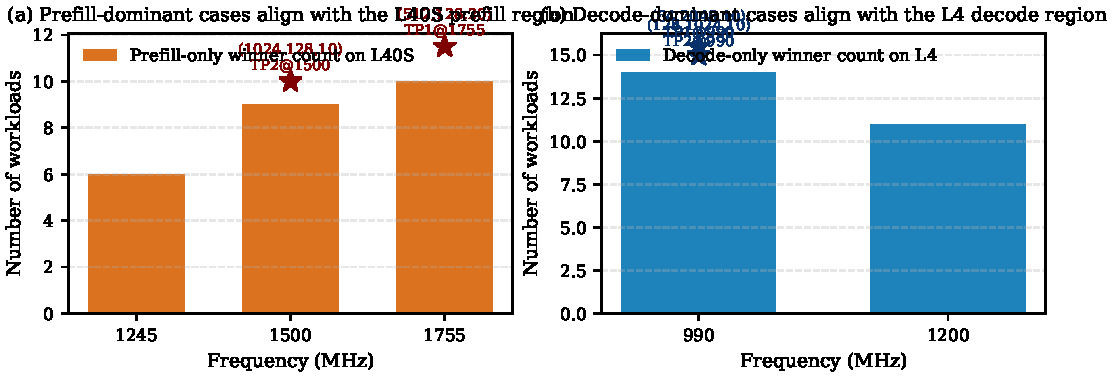
\includegraphics[width=\columnwidth]{figures/fig_obs2_phase_heterogeneity.pdf}
%   \caption{Observation 2 from experiments \texttt{A}--\texttt{D}.
%   Panel (a) aligns representative prefill-dominant monolithic winners from experiment \texttt{A} with the winner distribution from isolated prefill-only experiment \texttt{C}.
%   Panel (b) aligns representative decode-dominant monolithic winners from experiment \texttt{B} with the winner distribution from isolated decode-only experiment \texttt{D}.
%   The efficient operating region differs across phases, which motivates placing prefill and decode on different pools.}
%   \label{fig:obs2-phase-heterogeneity}
% \end{figure}

% The point of this observation is not simply that different GPUs have different raw performance.
% Rather, the measured operating regions suggest that the two inference phases map naturally to different pools.
% Experiments \texttt{C} and \texttt{D} provide the clearest evidence.
% In isolated prefill-only serving on the L40S, the energy-optimal frequency always lies between $1245$ and $1755$\,MHz across the 25 measured workloads, with winner counts concentrated at $1755$\,MHz for 10 workloads, $1500$\,MHz for 9 workloads, and $1245$\,MHz for 6 workloads.
% In isolated decode-only serving on the L4, the energy-optimal frequency is always either $990$ or $1200$\,MHz, with 14 workloads favoring $990$\,MHz and the remaining 11 favoring $1200$\,MHz.
% Thus, once the two phases are isolated, prefill and decode occupy clearly different efficient regions.

% Experiments \texttt{A} and \texttt{B} show that the same pattern already appears in end-to-end workloads.
% As shown in Fig.~\ref{fig:obs2-phase-heterogeneity}(a), the energy-optimal monolithic L40S points for prefill-dominant cases fall directly inside the prefill-only L40S winner region.
% For example, the prefill-heavy workload $(1024,128,r{=}10)$ is minimized at TP2 and $1500$\,MHz, while the mid-prefill workload $(512,128,r{=}20)$ is minimized at TP1 and $1755$\,MHz.
% Likewise, Fig.~\ref{fig:obs2-phase-heterogeneity}(b) shows that the energy-optimal \emph{monolithic L4} points for decode-dominant cases coincide with the decode-only L4 winner region.
% In experiment \texttt{B}, the decode-heavy workload $(128,1024,r{=}10)$ is minimized at TP2 and $990$\,MHz, and the very long decode workload $(64,2048,r{=}10)$ is minimized at TP1 and $990$\,MHz.

% This does not mean that L4 has universally higher decode throughput than L40S.
% The claim is narrower and more relevant to scheduling: prefill aligns with the efficient operating region of the L40S pool, whereas decode aligns with the efficient operating region of the L4 pool.
% This is exactly the asymmetry that SWEEP-LLM exploits through phase-aware routing.

% \subsection{Observation 2: The Knobs Interact}
% \label{sec:motivation:interaction}

% \begin{figure*}[t]
%   \centering
%   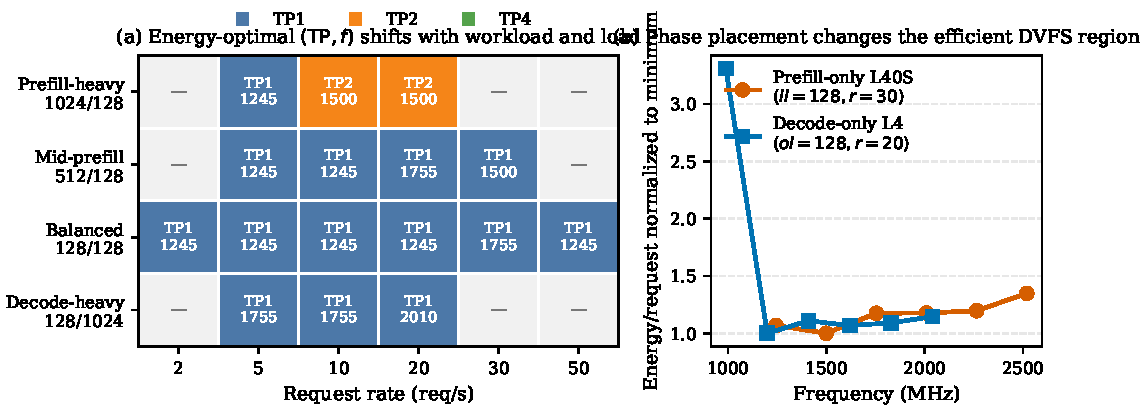
\includegraphics[width=\textwidth]{figures/fig_obs3_knob_interaction.pdf}
%   \caption{Observation 2 from experiments \texttt{A}, \texttt{C}, and \texttt{D}.
%   Panel (a) maps the energy-optimal $(\mathrm{TP}, f)$ in monolithic L40S serving across representative workload families and request rates.
%   Panel (b) shows representative phase-isolated DVFS curves for prefill on L40S and decode on L4.
%   The efficient TP and frequency depend jointly on workload mix, offered load, and phase placement.}
%   \label{fig:obs3-knob-interaction}
% \end{figure*}

% Observation~1 established that the best monolithic operating point changes across workloads.
% Experiment \texttt{A} further shows that the knobs change jointly rather than independently.
% Fig.~\ref{fig:obs3-knob-interaction}(a) maps the energy-optimal $(\mathrm{TP}, f)$ for rate sweeps on four workload families.
% Even within one token-shape family, the winner shifts with load.
% For the prefill-heavy family $(1024,128)$, the energy-optimal point moves from TP1 at $1245$\,MHz at $r{=}5$ to TP2 at $1500$\,MHz at $r{=}10$ and $r{=}20$.
% For the mid-prefill family $(512,128)$, TP1 remains preferred, but the best frequency changes from $1245$\,MHz at $r{=}5$ and $r{=}10$ to $1755$\,MHz at $r{=}20$ and then back to $1500$\,MHz at $r{=}30$.
% For the decode-heavy family $(128,1024)$, the best frequency shifts from $1755$\,MHz to $2010$\,MHz as load increases.
%
% Experiments \texttt{C} and \texttt{D} show that this coupling extends across phases.
% As shown in Fig.~\ref{fig:obs3-knob-interaction}(b), for isolated prefill on L40S with $(il{=}128,r{=}30)$, the minimum energy occurs at $1500$\,MHz, and running the same phase at $2520$\,MHz increases energy per request by $1.35\times$.
% For isolated decode on L4 with $(ol{=}128,r{=}20)$, the minimum occurs at $1200$\,MHz.
% Running that decode workload at $990$\,MHz increases energy per request by $3.31\times$, while running it at $2040$\,MHz still increases energy by $1.14\times$.
% Thus the efficient DVFS region depends on which phase is served, while the efficient TP depends on both load and token mix.
%
% These results rule out independent per-knob tuning.
% Once routing changes phase placement, the preferred TP and frequency change with it, and the routed load in turn determines how much capacity is needed on each pool.
% SWEEP-LLM therefore optimizes routing, TP, frequency, and active capacity jointly rather than through separate heuristics.

% Observation~1 showed that phase placement already changes the efficient hardware-frequency region.
% Observation~2 adds the next step: once routing, tensor parallelism, and frequency are all available, the locally optimal choice for one knob does not remain optimal after the others change.
% This is the core limitation of a decomposed controller such as DynamoLLM, which tunes knobs in stages on a homogeneous cluster.
% In our heterogeneous disaggregated setting, the knobs are coupled across pools and phases.

% Experiment \texttt{A} first shows that tensor parallelism and frequency are already coupled even without disaggregation.
% As shown in Fig.~\ref{fig:obs3-knob-interaction}(a), the prefill-heavy family $(1024,128)$ moves from TP1 at $1245$\,MHz at $r{=}5$ to TP2 at $1500$\,MHz at $r{=}10$ and $r{=}20$.
% The mid-prefill family $(512,128)$ keeps TP1, but its best frequency shifts from $1245$\,MHz to $1755$\,MHz and then back to $1500$\,MHz as the rate changes.
% Even within one workload family, the energy-optimal DVFS point therefore depends on the chosen TP and the offered load.

% Experiments \texttt{C} and \texttt{D} then show that routing couples into the same decision.
% In Fig.~\ref{fig:obs3-knob-interaction}(b), isolated prefill on L40S at $(il{=}128,r{=}30)$ is minimized at $1500$\,MHz, and moving to $2520$\,MHz increases energy per request by $1.35\times$.
% By contrast, isolated decode on L4 at $(ol{=}128,r{=}20)$ is minimized at $1200$\,MHz; running the same decode workload at $990$\,MHz increases energy by $3.31\times$, while $2040$\,MHz still costs $1.14\times$ more.
% Once routing changes which pool serves which phase, the efficient DVFS region changes with it.

% This coupling does not stop at the local phase level.
% Experiment \texttt{E} shows that combining individually sensible phase placements does not automatically yield a good end-to-end configuration: on the four representative workloads, the best disaggregated points still reach only $7.3\%$--$16.2\%$ of the throughput of the corresponding best monolithic points because KV-transfer and coordination overhead become part of the decision.
% Thus routing also interacts with active capacity and bundle sizing, not just with frequency.

% These results rule out independent per-knob tuning.
% In our setting, routing changes the load split across pools; that load split changes the desirable TP and frequency; and the resulting configuration determines whether disaggregation overhead can be amortized at all.
% SWEEP-LLM therefore schedules routing, tensor parallelism, frequency, and active capacity jointly rather than through separate per-knob heuristics.

% \subsection{Observation 3: Static Configurations and Blind Disaggregation Are Insufficient}
% \label{sec:motivation:static-fails}

% \begin{figure*}[t]
%   \centering
%   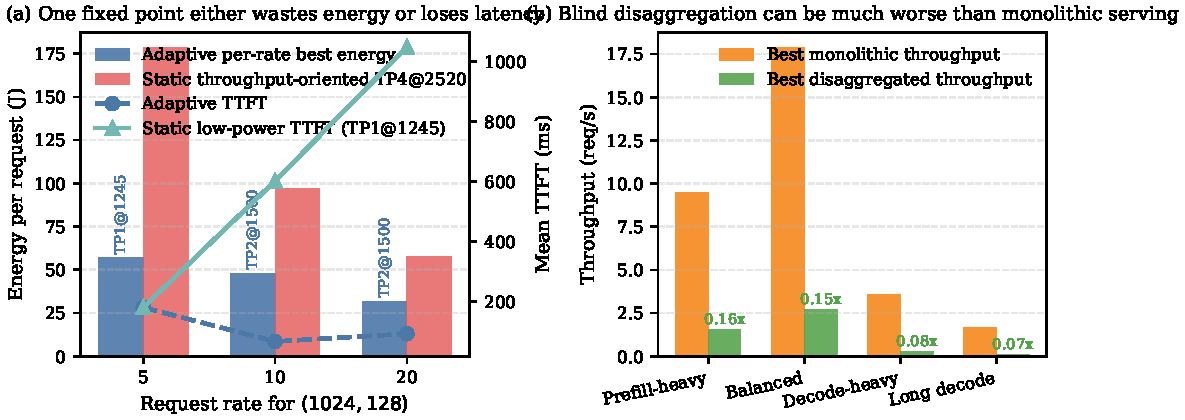
\includegraphics[width=\textwidth]{figures/fig_obs4_static_vs_disagg.pdf}
%   \caption{Observation 4 from experiments \texttt{A} and \texttt{E}.
%   Panel (a) shows that a fixed monolithic configuration cannot remain efficient across changing request rates.
%   Panel (b) compares the best disaggregated point from experiment \texttt{E} against the best monolithic point on the same representative workloads.
%   Efficient control therefore requires both online adaptation and explicit modeling of disaggregation overhead.}
%   \label{fig:obs4-static-disagg}
% \end{figure*}

% Experiments \texttt{A} and \texttt{E} show that neither a fixed configuration nor blind phase splitting is sufficient.
% Fig.~\ref{fig:obs4-static-disagg}(a) uses the prefill-heavy family $(1024,128)$ to illustrate the first failure mode.
% The static low-power point TP1 at $1245$\,MHz is energy-optimal only at $r{=}5$.
% When the arrival rate rises, its mean TTFT increases from $179.7$\,ms at $r{=}5$ to $601.2$\,ms at $r{=}10$ and $1047.4$\,ms at $r{=}20$.
% In contrast, the adaptive energy-optimal choice moves to TP2 at $1500$\,MHz at $r{=}10$ and $r{=}20$, keeping mean TTFT at $66.5$\,ms and $92.3$\,ms.
% The opposite extreme also fails.
% Using the static throughput-oriented point TP4 at $2520$\,MHz increases energy per request by $3.14\times$, $2.02\times$, and $1.82\times$ relative to the adaptive energy-optimal choice at $r{=}5$, $r{=}10$, and $r{=}20$, respectively.

% Fig.~\ref{fig:obs4-static-disagg}(b) shows the second failure mode.
% On the same four representative workloads used in Observations~1 and~2, the best disaggregated point from experiment \texttt{E} is still substantially worse than the best monolithic point.
% Its throughput reaches only $1.53$ versus $9.47$\,req/s on the prefill-heavy case, $2.72$ versus $17.87$\,req/s on the balanced case, $0.30$ versus $3.58$\,req/s on the decode-heavy case, and $0.12$ versus $1.65$\,req/s on the long-decode case.
% Disaggregation is therefore not automatically beneficial.
% Its specialization gain must exceed the KV-transfer and coordination overhead that splitting the phases introduces.

% These results motivate the online, state-aware control in SWEEP-LLM.
% The scheduler must update its operating point as workload state changes, and it must enable disaggregation only when the predicted benefit outweighs its overhead.
